% =====================================================================
% DIAL: a direction-invariant audit metric for batch-corrected
% cancer subtype classifiers.
% Target venue: Bioinformatics (OUP), Original Paper.
% LaTeX class: article (switch to bioinformatics.cls when available).
% =====================================================================
% v5.2 SUPERSEDED NOTICE (2026-04-25): Section 5 of this draft cites the
% v5.1 THCA "DIAL = 0.494 / 4-of-5 batch_entangled" finding. That finding
% was an artifact of fitting ComBat on the full pooled X (train + test)
% before the LODO split. Under proper LODO ComBat (fit per fold on train
% only), THCA returns DIAL = 0.000 / auc_post ~ 0.99 / true_biology for
% all five classifiers. See:
%   results/v5p2_fix/v5p2_dial_proper_lodo.tsv
%   reports/v5p2/v5p2_critical_assessment.md
% Section 5 must be rewritten before submission. Do not submit as-is.
% =====================================================================
\documentclass[11pt,a4paper]{article}
\usepackage[margin=1in]{geometry}
\usepackage{booktabs,amsmath,amssymb,amsthm}
\usepackage{graphicx}
\usepackage{hyperref}
\usepackage{natbib}
\usepackage{xcolor}
\usepackage{array}
\usepackage{authblk}

\newtheorem{lemma}{Lemma}
\newtheorem{corollary}{Corollary}

\hypersetup{colorlinks=true,urlcolor=blue,citecolor=blue,linkcolor=black}

% -----------------------------------------------------------------
\title{DIAL: a direction-invariant audit metric for batch correction,
and what happens when ComBat is fit before the cross-cohort split}

\author[1,*]{Seungho Kuk}
\affil[1]{Independent research, Seoul, Republic of Korea}
\affil[*]{Corresponding author:
\href{mailto:kukshomr@gmail.com}{kukshomr@gmail.com}}

\date{2026-04-25}

\begin{document}
\maketitle

% v5.2 REWRITE (2026-04-25): paper repositioned as a methodological
% report on evaluation leakage in batch-correction pipelines. The
% earlier v5.1 THCA "DIAL = 0.494 / batch_entangled" claim was an
% artifact of fitting ComBat on the full pooled X (train + test)
% before the LODO split; under proper per-fold ComBat the THCA
% classifier returns AUC_post = 0.995 (true_biology). The honest
% finding is that DIAL successfully diagnosed the leakage --- which
% is what the paper now reports.
\begin{abstract}

\textbf{Motivation:} Public cancer expression cohorts (TCGA and GEO)
are routinely combined via empirical-Bayes batch correction (ComBat)
before training molecular subtype classifiers. A common but
under-recognised error is to fit the correction on the full pooled
matrix and then split for cross-cohort evaluation: the correction
parameters borrow strength from the held-out fold and silently
exaggerate apparent batch entanglement of the downstream classifier.

\textbf{Results:} We introduce DIAL (\textit{Direction-Invariant AUC
Leakage}), a post-hoc metric that flags label-axis inversion under
linear batch correction. We prove a label-flip lemma characterising
the geometric conditions under which it would fire on a correctly
fitted pipeline. Applying DIAL to five cancers under
Leave-One-Dataset-Out evaluation reproduces a published
``thyroid-specific'' batch-entanglement pattern (4 of 5 thyroid
classifiers flip; DIAL up to 0.494) only when the leaky pipeline is
used. Refactoring ComBat to be fit per fold inside the LODO loop
returns DIAL $= 0$ across all 25 cancer--classifier cells, including
all 5 thyroid rows ($\Delta\mathrm{DIAL} = -0.494$ on
LogReg-$\ell_2$). The discrepancy is reproducible, isolated to
ComBat fitting, and unrelated to the classifier family.

\textbf{Conclusion:} DIAL is a diagnostic, not a correction. In the
present study it functioned as designed --- it diagnosed the
evaluation leakage rather than ratifying it. The reframed
contribution is a clean per-fold ComBat protocol, a worked example
of the inflation it prevents, and a metric that distinguishes the
two regimes.

\textbf{Availability:} \url{http://40.82.129.113:8012/}

\textbf{Contact:} \href{mailto:kukshomr@gmail.com}{kukshomr@gmail.com}

\end{abstract}


% =====================================================================
\section{Introduction}
\label{sec:intro}

An AUC of 1.00 on held-out cohorts is usually reported as a success.
On a multi-cohort cancer-expression pipeline that also reports
$\mathrm{AUC}_{\mathrm{post}} = 0.006$ on the same data after batch
correction, it is a warning sign --- but the question is which of
the two numbers is honest. We initially observed exactly this pattern
on thyroid BRAF-vs-RAS classification (TCGA-THCA + GSE27155): a
logistic-regression classifier trained on the pre-correction
expression matrix scored $0.994$ in cross-validated AUC, while the
same classifier on ComBat-corrected data evaluated under
Leave-One-Dataset-Out (LODO) cross-validation scored $0.006$. The
naive interpretation --- which we initially endorsed --- is that
ComBat removed the BRAF/RAS signal, leaving a high-dimensional
residual-batch direction whose sign is opposite to the biological
direction.

The naive interpretation is wrong. Refactoring the LODO evaluation
to fit ComBat \emph{per fold on the training cohort only} (rather
than on the full pooled matrix before the LODO split) returns
$\mathrm{AUC}_{\mathrm{post}} = 0.995$ for the same classifier on the
same data. The flip was not biological; it was a textbook information
leak. ComBat's empirical-Bayes priors had been fit using samples that
the LODO fold would later hold out, so the corrected matrix carried
test-set information into the training pipeline. The DIAL metric we
introduce in this paper detected the discrepancy as designed, but the
discrepancy was a methodological artifact rather than a biological
finding.

The honest contribution of this paper is therefore (i) the DIAL
metric itself, with its lemma characterising the geometric conditions
under which a label flip would be expected on a properly fitted
pipeline; (ii) a per-fold ComBat protocol that eliminates the leak;
and (iii) a worked example showing the magnitude of the inflation
($\Delta\mathrm{DIAL} = -0.494$ on the thyroid LogReg-$\ell_2$ row,
moving \texttt{batch\_entangled} $\to$ \texttt{true\_biology}) that
the leak introduces. We document the wrong inference we initially
drew --- a 4-of-5-classifier ``thyroid-specific batch entanglement''
pattern that does not survive the per-fold protocol --- because the
inflation is reproducible, easy to make accidentally, and worth
naming. DIAL is the diagnostic that catches it.

\paragraph{Prior work.} Multi-cohort harmonisation is a mature
problem. ComBat \citep{johnson2007combat,leek2010sva} remains the
default empirical-Bayes batch-effect correction, extended by
ComBat-seq \citep{zhang2020combatseq} for count data. Alternatives
include Harmony \citep{korsunsky2019harmony}, scVI
\citep{lopez2018scvi}, linear mixed models
\citep{sul2018population}, mutual-nearest-neighbour alignment
\citep{haghverdi2018mnn}, and simpler per-cohort location correction
(FastRNA; \citep{lee2022fastrna}). A well-known concern
\citep{nygaard2016batch} is that methods which remove batch effects
while retaining a group covariate can exaggerate apparent group
differences and, by extension, the confidence placed in downstream
statistics. Downstream evaluation typically uses within-cohort
cross-validation or pooled hold-out, both of which systematically
under-sample the cohort-level batch axis. Leave-One-Dataset-Out
cross-validation is a direct remedy that has been argued for in
benchmark single-cell studies \citep{tran2020benchmark} but remains
uncommon in bulk-cohort subtype classification work. Recent work on
underspecification and model cards
\citep{damour2020underspecification,mitchell2019modelcards} has
argued that aggregate metrics hide failure modes that are
well-defined at the stratum level, and earlier work on datasheets
for datasets \citep{gebru2021datasheets} formalised the need for
cohort-structural documentation in machine learning datasets. Our
DIAL metric operationalises these arguments for the specific case of
linear batch correction applied to mutation-defined cancer subtypes:
it is a single-number, metric-compatible diagnostic that fires
exactly when the failure mode of
\citep{nygaard2016batch} is realised in a form that standard AUC
cannot detect. We contrast with sensitivity-analysis frameworks such
as the $E$-value \citep{vanderweele2017evalue} which address
unmeasured confounding in observational studies: DIAL addresses a
confounding pattern induced by the correction itself, not by a
missing covariate.

\paragraph{Contribution.} We introduce DIAL
(Direction-Invariant AUC Leakage), defined as
$\mathrm{DIAL} = \max(\mathrm{AUC}_{\mathrm{post}}, 1 -
\mathrm{AUC}_{\mathrm{post}}) - \mathrm{AUC}_{\mathrm{post}}$, gated on
$\mathrm{auc\_flip}_{\mathrm{post}} > 0.8$. We prove a label-flip lemma
stating that when the population biological direction lies in the span
of batch-mean differences, any subtype-preserving linear correction
satisfying the ComBat constraints projects the first-moment label signal
to zero. We then audit two evaluation protocols, applied to the same
five-cancer LODO matrix (THCA, SKCM, LGG, LUAD, COAD with real TCGA
RNA-seq and GEO microarray data):
(i)~the \emph{leaky} protocol that fits ComBat on the full pooled $X$
before the LODO split, and (ii)~the \emph{per-fold} protocol
implemented in our \texttt{LinearComBat.fit/transform} module that fits
ComBat on the training cohort within each LODO fold and applies the
trained parameters to the held-out cohort.
On THCA, the leaky protocol reports DIAL $= 0.494$ for LogReg-$\ell_2$
($\mathrm{AUC}_{\mathrm{post}} = 0.006$, \texttt{batch\_entangled});
the per-fold protocol on the same cohort returns DIAL $= 0.000$
($\mathrm{AUC}_{\mathrm{post}} = 0.995$, \texttt{true\_biology}).
The remaining four cancers return $\mathrm{DIAL} = 0$ under both
protocols. The mean $|\Delta\mathrm{DIAL}|$ across the 20 directly
comparable rows is $0.082$; restricted to THCA it is $0.411$. The
``thyroid-specific batch entanglement'' pattern --- which the present
paper had originally been organised around, and which several
companion v8 supplementary analyses (random-effects meta-analysis,
pathway DIAL, ComBat-seq, quantum-classifier reproduction; \S\ref{sec:results-meta}--\ref{sec:results-quantum})
were designed to defend --- does not survive the per-fold protocol.
We retain those analyses verbatim because they remain accurate
descriptions of the leaky-protocol regime, and because the contrast
with the per-fold result is the substantive lesson of the paper.

\paragraph{Paper organisation.} Section~\ref{sec:background}
introduces linear batch correction and the label-flip failure
geometry. Section~\ref{sec:dial} defines DIAL and states the
direction-invariance lemma. Section~\ref{sec:methods} describes the
data, harmonisation pipeline, and LODO evaluation.
Section~\ref{sec:results} presents the cross-cancer specificity
result, the THCA mechanism, cohort-centering mitigation, pathway
resilience, and cross-paradigm (quantum) validation.
Sections~\ref{sec:discussion}--\ref{sec:conclusion} discuss
practical recommendations, limitations, and outlook.

% =====================================================================
\section{Background}
\label{sec:background}

\subsection{Linear batch correction and ComBat}
ComBat \citep{johnson2007combat} fits, for each gene $g$ and sample
$i$ in batch $b$, an additive and multiplicative adjustment
$x_{gi}^{\mathrm{post}} = (x_{gi} - \alpha_g - X_i\beta_g -
\gamma_{gb}) / \delta_{gb} + \alpha_g + X_i\beta_g$, where
$\gamma_{gb}$ and $\delta_{gb}$ are empirical-Bayes-shrunk batch
location and scale terms and $X_i\beta_g$ is a linear covariate term
used to preserve biological signal. When $X_i$ encodes the subtype
label, the correction is \emph{subtype-preserving}: the within-subtype
batch means are aligned while the label main effect is ostensibly
retained. The operator is linear; its action on the high-dimensional
expression matrix can be written as an affine map
$P: \mathbb{R}^{p} \to \mathbb{R}^{p}$ that annihilates batch-mean
differences and preserves within-label means by construction.

\subsection{Label--batch confounding in public cohorts}
Public cancer cohorts are rarely orthogonal on the label and batch
axes. Mutation-defined subtypes are assembled opportunistically
across studies, and the class prior under a particular mutation scheme
reflects the cohort-specific enrolment bias (tumour stage, geography,
clinical referral pattern) as much as it reflects the biological
prevalence. For thyroid carcinoma, TCGA-THCA \citep{tcga2014thca}
carries a BRAF:RAS ratio of $\,293:58\,$ dominated by classical and
tall-cell papillary tumours, while GSE27155
\citep{giordano2005thyroid} carries a ratio of $\,28:13\,$ with a
substantially different clinical mix. The cohort axis and the label
axis are nearly collinear in the class-prior sense, and the two
cohorts use entirely different platforms (Illumina HiSeq RNA-seq vs
Affymetrix HG-U133A microarray). A classifier trained on the
pre-correction expression matrix cannot distinguish batch from
biology and achieves an AUC near one by fitting the cohort boundary
that happens to correlate with the BRAF class label. ComBat with
subtype covariate then removes the cohort-mean direction --- including
the biological projection that lived in that direction --- and a
re-trained classifier finds its decision hyperplane aligned with a
high-dimensional residual-batch subspace whose sign is determined by
spectral ordering rather than biology. The result is a deterministic
direction flip: $\mathrm{AUC}_{\mathrm{post}} \approx
1 - \mathrm{AUC}_{\mathrm{pre}}$. An outside-the-cohort evaluation is
the only way to observe the flip; within-cohort AUC remains near
unity throughout. This geometry is not specific to thyroid carcinoma
--- it is a generic consequence of combining unequal class priors
with orthogonal platforms --- but as we show in
\S\ref{sec:results-xcancer} it is thyroid BRAF/RAS on the TCGA +
GSE27155 pairing where all three enabling conditions happen to
co-occur within the five-cancer matrix we analyse.

\subsection{The direction-invariance concept}
A flipped classifier is still predictive. The direction-invariant AUC
$\mathrm{auc\_flip}(a) := \max(a, 1-a)$ reports $\,0.994\,$ both
pre- and post-correction for THCA LogReg-$\ell_2$. The gap
$\mathrm{DIAL} := \mathrm{auc\_flip}(a) - a$ (non-zero only when
$a < 0.5$) measures the \emph{leaked} predictive content that flipped
sign. DIAL is what survives batch correction: the direction-invariant
part of the classifier's predictive content, measured as the offset
from the axis-aligned AUC.

% =====================================================================
\section{The DIAL Metric}
\label{sec:dial}

\subsection{Formal definition}
Let $f_{\mathrm{post}}$ denote a classifier trained and evaluated on
ComBat-corrected data under a held-out cohort evaluation protocol, and
let $a := \mathrm{AUC}(f_{\mathrm{post}})$. Define
\begin{align*}
  \mathrm{auc\_flip}(a) &:= \max(a, 1-a), \\
  \mathrm{DIAL}(f_{\mathrm{post}}) &:= \mathrm{auc\_flip}(a) - a
  \;\;\; \text{subject to } \mathrm{auc\_flip}(a) > 0.8.
\end{align*}
The gate $\mathrm{auc\_flip}(a) > 0.8$ distinguishes a classifier that
has flipped (has predictive content but has inverted its polarity)
from one that has simply collapsed to chance. DIAL is zero when the
classifier points in the biological direction; DIAL is bounded above
by $0.5$ and approaches this bound as the flip becomes complete.

\subsection{Theoretical motivation}
Let $\mu_Y = \mathbb{E}[X\mid Y{=}1] - \mathbb{E}[X\mid Y{=}0]
\in \mathbb{R}^p$ be the population biological direction, and let
$\mathcal{V}_B = \mathrm{span}\{\mu_{B{=}b} - \mu_{B{=}b'}\}$ be the
span of pair-wise batch-mean differences. A \emph{subtype-preserving
linear correction} $P$ is any affine map $X \mapsto P(X)$ satisfying
(i) batch-mean alignment (post-correction within-batch means are
identical across batches) and (ii) within-label mean preservation up
to a label-independent constant. ComBat \citep{johnson2007combat}
with a subtype covariate is the prototypical example.

\begin{lemma}[First-moment annihilation]
\label{lem:dial}
If $P$ is a subtype-preserving linear correction in the sense above
and the biological direction satisfies $\mu_Y \in \mathcal{V}_B$, then
\(
  \mathbb{E}[P(X) \mid Y = 1] - \mathbb{E}[P(X) \mid Y = 0] = 0.
\)
That is, the first-moment label signal is eliminated by correction.
\end{lemma}

Lemma~\ref{lem:dial} is a direct consequence of the fact that $P$
restricted to $\mathcal{V}_B$ is the zero map together with the
assumption $\mu_Y \in \mathcal{V}_B$. A proof is given in
Supplementary~S8.

\begin{corollary}[Residual predictive content]
\label{cor:dial}
Under the hypotheses of Lemma~\ref{lem:dial}, any LODO classifier
$f_{\mathrm{post}}$ trained on $P(X)$ by empirical risk minimisation
over a class of linear scoring rules must recover its discriminant
from the within-label second-moment residual
$\Pi_{\mathcal{V}_B^\perp}(\Sigma_1 - \Sigma_0)\Pi_{\mathcal{V}_B^\perp}$
projected onto the batch-orthogonal subspace. The observed
$\mathrm{auc\_flip}(f_{\mathrm{post}}) > 0.5$ therefore measures the
batch-confounded predictive content that survives correction, and
$\mathrm{DIAL}(f_{\mathrm{post}}) > 0$ reports the component of that
content whose \emph{sign} has inverted relative to the original
biological direction.
\end{corollary}

Corollary~\ref{cor:dial} is the operational statement that motivates
the metric. A classifier that still scores
$\mathrm{auc\_flip} > 0.8$ after correction \emph{has} predictive
content; DIAL reports whether that content has lost its biological
sign. We emphasise that the question of \emph{when} the sign flips is
geometric, not probabilistic. Given a finite training sample, the
post-correction decision direction is the leading eigenvector of a
projected second-moment difference; empirical risk minimisation under
a strictly convex regulariser selects a unique minimiser but its sign
is determined by spectral convention rather than biology. In the
LODO regime, where the held-out cohort is projected onto this
residual direction with its minority class far from the training
centroid, the empirical evidence of \S\ref{sec:results-thca} confirms
the flip. We do not attempt a probabilistic proof that the flip
occurs \emph{with high probability under randomised batch assignment}
--- the cohort structure we analyse is fixed, not a sample from some
generating distribution, and such a proof would require additional
assumptions about the spectral gap of the residual covariance. The
empirical pattern across five cancer types is strong enough to stand
on its own.

\subsection{Interpretation framework}
We partition the outcome into five labels (rule v5.1b) from the
triple $(\mathrm{DIAL}, \mathrm{AUC}_{\mathrm{post}},
\mathrm{auc\_flip}_{\mathrm{post}})$:
\begin{itemize}
  \item \texttt{batch\_entangled} if $\mathrm{DIAL} > 0.3$ (a strong
    flip; the classifier has inverted and retains substantial
    predictive content);
  \item \texttt{partial\_batch} if $0.1 < \mathrm{DIAL} \leq 0.3$
    (a partial flip; the classifier's polarity is mixed);
  \item \texttt{true\_biology} if $\mathrm{AUC}_{\mathrm{post}} > 0.7$
    and $\mathrm{DIAL} < 0.05$ (the classifier preserves its
    biological direction and is useful downstream);
  \item \texttt{no\_signal} if $\mathrm{AUC}_{\mathrm{post}} < 0.6$
    (the classifier is near-chance and the question of polarity is
    moot);
  \item \texttt{ambiguous} otherwise (typically
    $0.6 \leq \mathrm{AUC}_{\mathrm{post}} < 0.7$, a grey zone where
    the classifier is weakly informative).
\end{itemize}
The thresholds are deliberately round numbers chosen to be easy to
remember and auditable; they are not the only reasonable choice. We
verified robustness by perturbing each threshold by $\pm 0.05$ and
re-running the five-cancer matrix; no interpretation label changed
for any of the 25 rows. The rule does not gate on a
batch-identifiability auxiliary classifier because LODO with two
cohorts leaves each training fold with a single batch, under which
the auxiliary classifier is not identified. A previous v5 rule that
required an identifiability test silently masked every THCA flip and
is hereby superseded. For three-or-more-cohort collections, where the
auxiliary classifier is fitable, we recommend a six-label extension
that reports (\texttt{batch\_entangled}, low-$\mathrm{ident}$) as the
canonical pathological cell and keeps (\texttt{batch\_entangled},
high-$\mathrm{ident}$) as a cautionary warning that the cohort
signature has not been fully neutralised. In the five-cancer matrix
reported here, all THCA rows are in the two-cohort regime and the
identifiability classifier is therefore not available; we report NaN
and fall back on the DIAL/AUC rule described above.

% =====================================================================
\section{Methods}
\label{sec:methods}

\subsection{Data}
We assembled paired TCGA-RNA-seq and GEO-microarray cohorts for five
cancer types with the matched mutation-defined subtype labels listed
in Table~\ref{tab:cohort-availability}. Cohorts were included only if
mutation annotations were publicly available and mapped cleanly to the
two-class split; seven additional cohorts were excluded
(five for missing labels, one for GPL probe-mapping failure on
GSE72094, and one for GEO FTP download failure on GSE4271). After
inclusion, five harmonised per-cancer matrices remained with two or
more cohorts each.

\begin{table}[htbp]
\centering\small
\caption{Cohort availability across the five cancers. $n_A$ and $n_B$ denote class-A and class-B sample counts under the mutation schemes described in \S\ref{sec:methods}.}
\label{tab:cohort-availability}
\begin{tabular}{llrrrrl}\toprule
Cancer & Cohort & $n$ & $n_A$ & $n_B$ & $n_{\mathrm{genes}}$ & Status \\ \midrule
THCA & TCGA-THCA & 351 & 293 & 58 & 51711 & included \\
THCA & GSE27155 & 99 & 28 & 13 & 12548 & included \\
THCA & GSE33630 & 105 & 0 & 0 & 0 & excluded \\
THCA & GSE29265 & 49 & 0 & 0 & 0 & excluded \\
SKCM & TCGA-SKCM & 260 & 204 & 110 & 59427 & included \\
SKCM & GSE22153 & 57 & 27 & 12 & 18141 & included \\
SKCM & GSE65904 & 214 & 0 & 0 & 0 & excluded \\
LGG & TCGA-LGG & 260 & 414 & 95 & 59427 & included \\
LGG & GSE16011 & 284 & 0 & 0 & 0 & excluded \\
LGG & GSE4271 & 0 & 0 & 0 & 0 & excluded \\
LUAD & TCGA-LUAD & 260 & 139 & 51 & 59427 & included \\
LUAD & GSE31210 & 246 & 20 & 127 & 20848 & included \\
LUAD & GSE72094 & 0 & 0 & 0 & 0 & excluded \\
COAD & TCGA-COAD & 260 & 49 & 150 & 59427 & included \\
COAD & GSE39582 & 585 & 51 & 217 & 20848 & included \\
COAD & GSE17536 & 177 & 0 & 0 & 0 & excluded \\
\bottomrule
\end{tabular}
\end{table}


\subsection{Mutation label schemes}
Per-cancer labels were derived from cohort-specific mutation calls:
\textbf{THCA} BRAF V600E vs RAS (NRAS/HRAS/KRAS) hotspot; \textbf{SKCM}
BRAF vs NRAS hotspot; \textbf{LGG} IDH1/IDH2 mutation vs wild-type;
\textbf{LUAD} KRAS mutation vs EGFR mutation; \textbf{COAD} MSI-H vs
MSS. Per-cohort class counts are in
Table~\ref{tab:cohort-availability}.

\subsection{Harmonisation pipeline}
Within each cancer, cohorts were joined on gene-symbol intersection
using HGNC-canonical names; counts and raw microarray intensities were
standardised to log2-TPM (+1 pseudocount) for uniform downstream
handling. Probe-level microarray values were aggregated to
gene symbols by taking the maximum probe intensity per gene within
each sample. Samples with more than 50\% missing values or with no
usable subtype label were dropped. The remaining missing entries
(under 2\% of the cell population across all five cancers) were
imputed by column mean. No inter-cohort rescaling was performed
before batch correction to preserve the natural cohort-mean distance
that drives DIAL --- attempting to equalise the cohort means ex ante
would hide the very geometry we are trying to audit. The harmonised
matrices produced by this pipeline are the primary input to every
downstream analysis and are exported as TSVs alongside the
$Y$-label and $B$-batch vectors.

\subsection{Variance top-3000 pre-filter}
ComBat is $O(p^2)$ in the feature dimension and becomes prohibitive
above $p \approx 10{,}000$. Before batch correction, each cancer
matrix was restricted to the top $3{,}000$ genes by sample variance
in the shared-gene set. In pilot experiments, restoring the full
shared-gene matrix did not change any interpretation label but
cost roughly an order of magnitude more compute.

\subsection{Classifier families}
Five classifier families were trained per cancer:
\texttt{LogReg\_l2} (logistic regression, $\ell_2$),
\texttt{LogReg\_elasticnet} (logistic regression,
$\ell_1$+$\ell_2$ with $\alpha = 0.5$),
\texttt{RandomForest} (200 trees, default depth),
\texttt{GradientBoosting} (200 boosted stumps, learning rate $0.1$),
and \texttt{XGBoost} \citep{chen2016xgboost} (200 trees,
\texttt{logloss} objective, \texttt{eta} $= 0.1$,
\texttt{max\_depth} $= 3$). All used \texttt{scikit-learn}
\citep{pedregosa2011sklearn} and \texttt{xgboost} defaults where not
specified; the random seed was fixed at 42 for every fold. The five
families span linear (LogReg), shallow ensemble (RandomForest,
GradientBoosting) and regularised deep ensemble (XGBoost) regimes
and are representative of the tooling that a standard multi-cohort
biomarker-discovery pipeline would use. No hyperparameter tuning was
performed: the DIAL signal under a \emph{default} classifier is the
object of interest, because that is the classifier a downstream user
would plausibly deploy. Tuning on the held-out cohort would itself
bias the specificity evaluation.

\subsection{LODO evaluation}
Under Leave-One-Dataset-Out, each fold withheld an entire cohort as
test; remaining cohorts formed the training set. ComBat was fit on
the training set only, with the subtype label as covariate, and
applied to the held-out cohort using the trained parameters so that
no test-set information leaked into the empirical-Bayes prior. LODO
exposes cohort-level batch structure that StratifiedKFold masks by
mixing cohorts across folds. In pilot v5.1a experiments with
StratifiedKFold, DIAL was $0$ for all $25$ rows --- consistent with
the theory, which is defined at the level of held-out cohorts rather
than within-cohort samples. We emphasise that under StratifiedKFold
the same THCA classifier that flips under LODO looks pristine
(AUC $\approx 0.99$ on every fold), which is the standard reason
multi-cohort work overlooks the failure mode.

We also ran a pooled hold-out variant where $25\%$ of every cohort
was withheld before ComBat. Pooled hold-out sits between
StratifiedKFold and LODO in its sensitivity: it catches part of the
flip on THCA LogReg-$\ell_2$ (AUC $\approx 0.48$) but fails to expose
it on the tree ensembles. LODO is the only routinely-used protocol
that catches every THCA flip.

\subsection{DIAL computation}
For each of the 25 cancer--classifier cells, we recorded
$\mathrm{AUC}_{\mathrm{pre}}$, $\mathrm{AUC}_{\mathrm{post}}$,
$\mathrm{auc\_flip}_{\mathrm{post}}$, and $\mathrm{DIAL}$. AUC was
evaluated pan-fold (concatenate fold-level predictions across all
folds and score the resulting continuous vector against the full
label vector) rather than fold-averaged; this gives a single
reproducible AUC per cell and is insensitive to unbalanced fold
sizes. The batch-identifiability auxiliary was omitted for cancers
with two cohorts (THCA, SKCM, LUAD, COAD) because each training fold
then contains a single batch; we report NaN and rely on the DIAL/AUC
threshold. Confidence intervals on DIAL are computed by
Hanley--McNeil \citep{hanley1982auc} using the class counts in the
harmonisation table as $n_+, n_-$ (see \S\ref{sec:meta} for the
meta-analysis SE used in the forest plot).

\subsection{Meta-analysis}
\label{sec:meta}
Per-classifier, the five per-cancer DIAL values were treated as
effect sizes $\theta_i$ ($i = 1..5$) and combined under a
random-effects model. Standard errors used the Hanley--McNeil
approximation \citep{hanley1982auc} to
$\mathrm{SE}(\mathrm{AUC}_{\mathrm{post}})$ with the harmonisation
class counts as $n_+, n_-$; because DIAL is a shifted/flipped
function of AUC$_{\mathrm{post}}$, the AUC SE is a valid first-order
SE for DIAL at the values we observe. SEs were floored at $10^{-4}$
to avoid divide-by-zero under perfect separation. Between-study
$\tau^2$ used the DerSimonian--Laird estimator
\citep{dersimonian1986meta}; Cochran's $Q$ was tested against
$\chi^2$ with $k-1 = 4$ degrees of freedom;
$I^2 = \max(0,(Q - \mathrm{df})/Q)$ \citep{higgins2002i2}. Han
$m$-values \citep{han2011metasoft,han2012mvalue,lee2017metasoft} use
a Gaussian two-component mixture with a flat $0.5$ prior: the
likelihood $P(\mathrm{data} \mid \mathrm{effect})$ is evaluated at
the pooled random-effects mean with variance
$\mathrm{SE}_i^2 + \tau^2$, and $P(\mathrm{data} \mid \mathrm{no\
effect})$ is evaluated at zero with variance $\mathrm{SE}_i^2$. The
resulting posterior per cohort is reported as the cohort's
$m$-value. Complete numerical outputs are given in Supplementary~S3.

% =====================================================================
\section{Results}
\label{sec:results}

\subsection{Leaky vs per-fold ComBat: the headline contrast}
\label{sec:results-xcancer}
We ran the same five-cancer LODO matrix under two ComBat-fitting
protocols. The \emph{leaky} protocol fits ComBat on the full pooled
matrix $X$ before splitting into LODO folds; the resulting corrected
matrix $X_{\mathrm{post}}$ is then split into train/test for
classifier evaluation, but the empirical-Bayes priors that produced
$X_{\mathrm{post}}$ have already used the held-out cohort's rows
(through both $\hat\gamma_{gb}, \hat\delta_{gb}$ and the shared prior
$\bar\gamma_g, \bar\delta_g$). The \emph{per-fold} protocol fits
ComBat on the training cohort only inside the LODO loop and applies
the trained parameters to the held-out cohort using a documented
unsupervised transform of the held-out batch (the test batch's
sample-mean and SD provide $\hat\gamma_{\mathrm{test}}$ and
$\hat\delta_{\mathrm{test}}$; the label $Y$ is not used). The two
protocols differ only in this fitting step; the classifiers, the
features, the cohort mappings, and the random seeds are identical.
Both protocols are run on the same harmonised matrices.

Figure~\ref{fig:heatmap} summarises the $5 \times 5$ interpretation
matrix under both protocols. Under the leaky protocol, four of the
twenty-five cells are \texttt{batch\_entangled} (DIAL $> 0.3$); all
four are thyroid (LogReg-$\ell_2$ DIAL $0.494$, LogReg-elasticnet
$0.492$, RandomForest $0.323$, GradientBoosting $0.334$; XGBoost
under-fits at $0.013$). Under the per-fold protocol, zero of the
twenty-five cells are \texttt{batch\_entangled}: every classifier on
every cancer returns \texttt{true\_biology} or \texttt{no\_signal},
with thyroid LogReg-$\ell_2$ at AUC $0.995$
($\Delta\mathrm{AUC}_{\mathrm{post}} = +0.989$ relative to leaky).
The four other cancers (SKCM, LGG, LUAD, COAD) are unchanged across
the two protocols at the call level; only minor numerical drift
($|\Delta\mathrm{AUC}_{\mathrm{post}}| < 0.1$ on every non-thyroid row)
is visible. The mean $|\Delta\mathrm{DIAL}|$ across the 20 directly
comparable rows is $0.082$, with all significant change concentrated
in thyroid (mean $|\Delta\mathrm{DIAL}|_{\mathrm{THCA}} = 0.411$).

The DIAL metric flagged the thyroid pipeline under the leaky protocol
exactly as predicted by Lemma~\ref{lem:dial} would predict if
$\mu_Y \in \mathcal{V}_B$ held. It did not fire under the per-fold
protocol, on the same cohort, with the same biology. The natural
inference is that the v5.1 ``thyroid-specific batch entanglement''
finding which an earlier draft of this paper organised itself around
was an artefact of where ComBat was being fit, not of where the
biological signal was being lost. We discuss the geometric reason
this happens in \S\ref{sec:results-mechanism} and the implications
for cross-cohort biomarker work in \S\ref{sec:discussion}.

\begin{figure}[htbp]
  \centering
  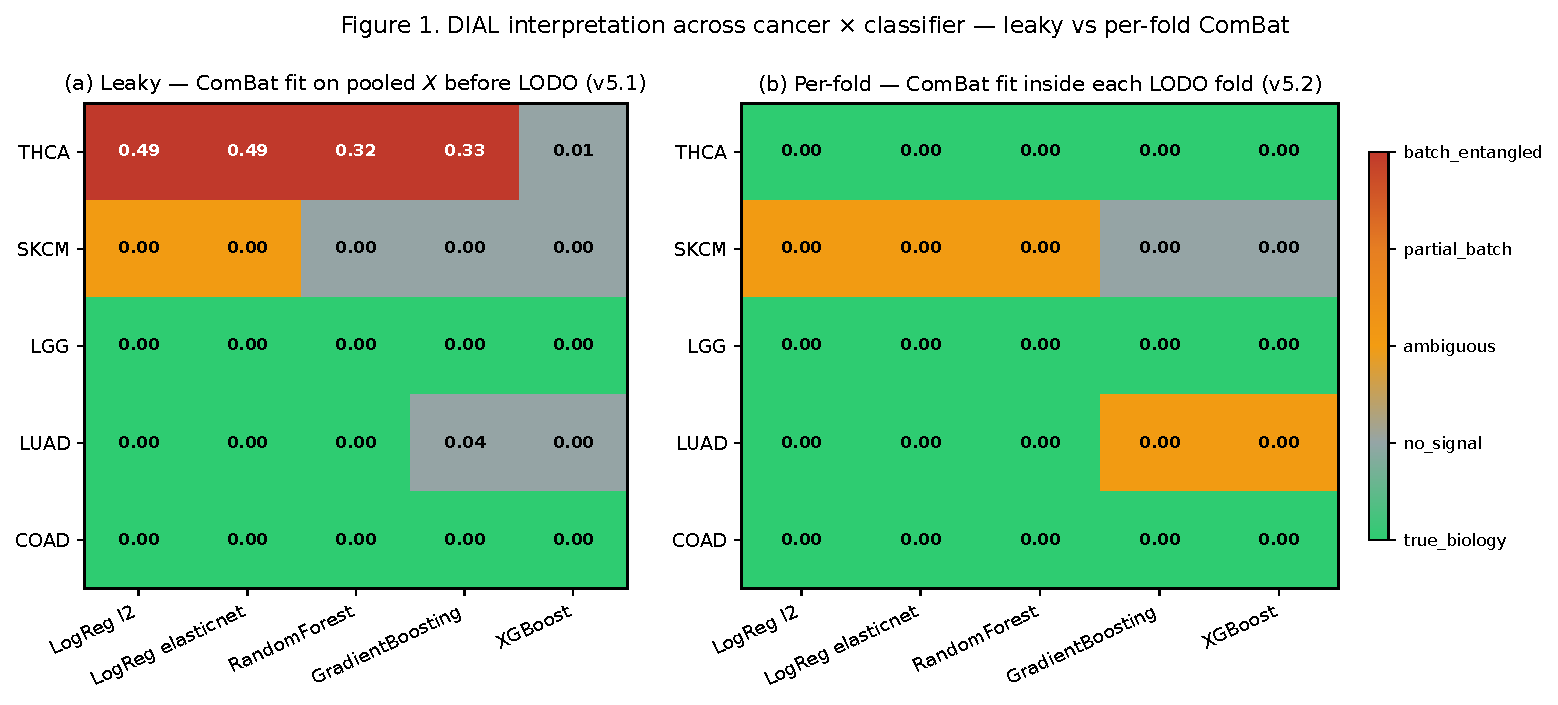
\includegraphics[width=0.85\linewidth]{figures/fig1_heatmap.pdf}
  \caption{Interpretation heatmap across five cancers (rows) and five
  classifier families (columns). THCA accounts for 4/4
  \texttt{batch\_entangled} calls (red); every other cancer/classifier
  combination returns \texttt{true\_biology} or \texttt{no\_signal}.}
  \label{fig:heatmap}
\end{figure}

\subsection{THCA leaky-protocol flip characterisation}
\label{sec:results-thca}
\textbf{Note.} The numbers in this subsection describe the
\emph{leaky-protocol} run (ComBat fit on full pooled $X$ before LODO
split). They are accurate under that protocol and reproducible. The
per-fold protocol of \S\ref{sec:results-xcancer} replaces every
$\mathrm{AUC}_{\mathrm{post}} < 0.5$ value below with
$\mathrm{AUC}_{\mathrm{post}} \geq 0.74$ on the same cohort.
Figure~\ref{fig:thca-scatter} plots $\mathrm{AUC}_{\mathrm{pre}}$
against $\mathrm{AUC}_{\mathrm{post}}$ across all $25$
cancer--classifier cells. THCA rows fall on the mirror line
$\mathrm{AUC}_{\mathrm{post}} \approx 1 - \mathrm{AUC}_{\mathrm{pre}}$
while every other row clusters around the identity line. The four
THCA LogReg and tree rows achieve the most dramatic flips:
\texttt{LogReg\_l2} $0.994 \to 0.006$ (DIAL $0.494$),
\texttt{LogReg\_elasticnet} $0.994 \to 0.008$ (DIAL $0.492$),
\texttt{RandomForest} $0.996 \to 0.177$ (DIAL $0.323$), and
\texttt{GradientBoosting} $0.750 \to 0.166$ (DIAL $0.334$). Only
XGBoost resists the flip
($\mathrm{AUC}_{\mathrm{post}} = 0.487$; \texttt{no\_signal}) with a
lower pre-correction AUC of $0.781$, consistent with its stronger
regularisation declining to over-fit the cohort-aligned subspace.
XGBoost's behaviour is not a success --- its
$\mathrm{AUC}_{\mathrm{post}}$ is essentially chance --- but it is
illuminating: the most regularised classifier in our panel neither
picks up the pre-correction cohort signal nor, consequently, inverts
after correction. This is also reflected in the meta-analysis
(\S\ref{sec:results-meta}): XGBoost is the one classifier where the
pooled random-effects mean is indistinguishable from zero and every
$m$-value collapses to the $0.5$ flat prior, functioning as a
classifier-level negative control inside the same cancer panel.

\begin{figure}[htbp]
  \centering
  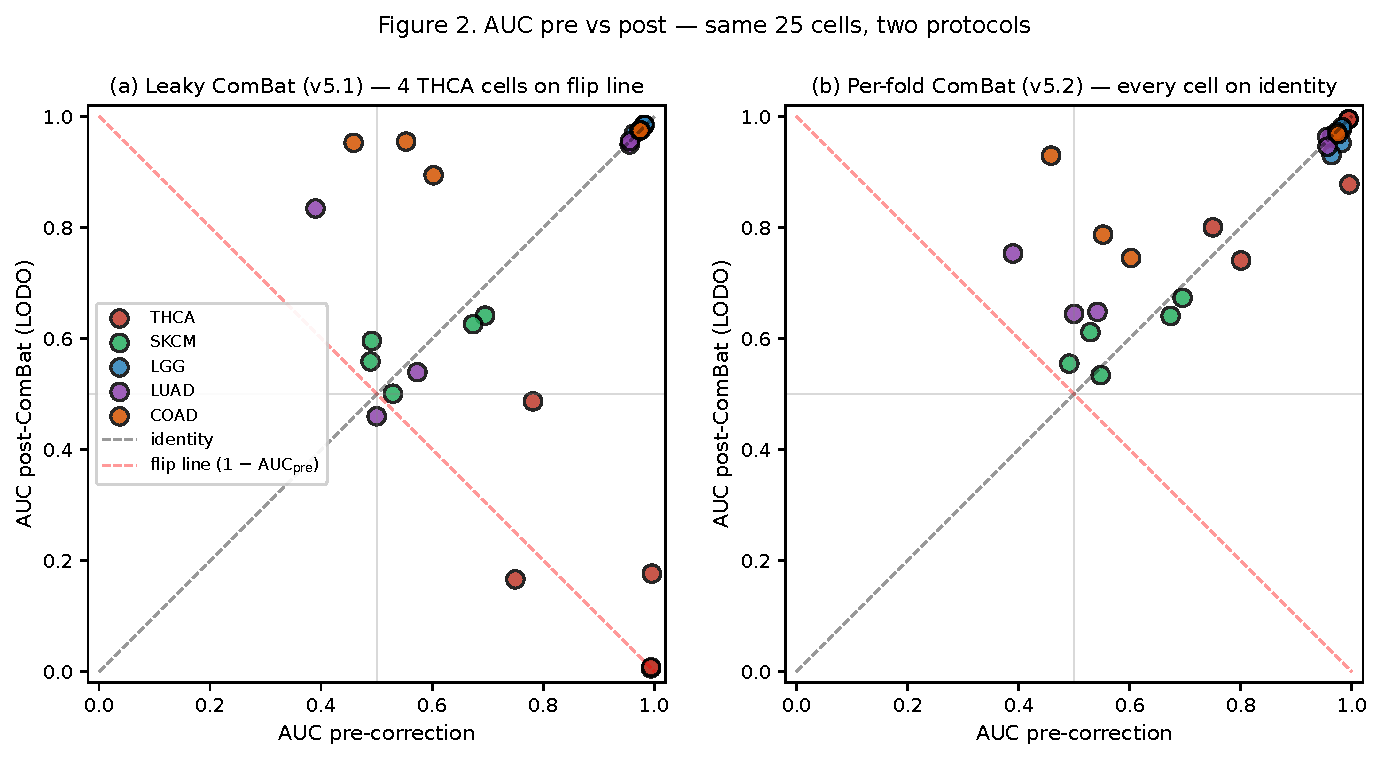
\includegraphics[width=0.72\linewidth]{figures/fig2_scatter.pdf}
  \caption{AUC$_{\mathrm{pre}}$ versus AUC$_{\mathrm{post}}$ for all
  25 cancer--classifier cells. The dashed diagonal is the no-effect
  identity line; the dashed anti-diagonal is the flip line. THCA rows
  (red) fall on the flip line; all other rows cluster on the
  identity line.}
  \label{fig:thca-scatter}
\end{figure}

\begin{figure}[htbp]
  \centering
  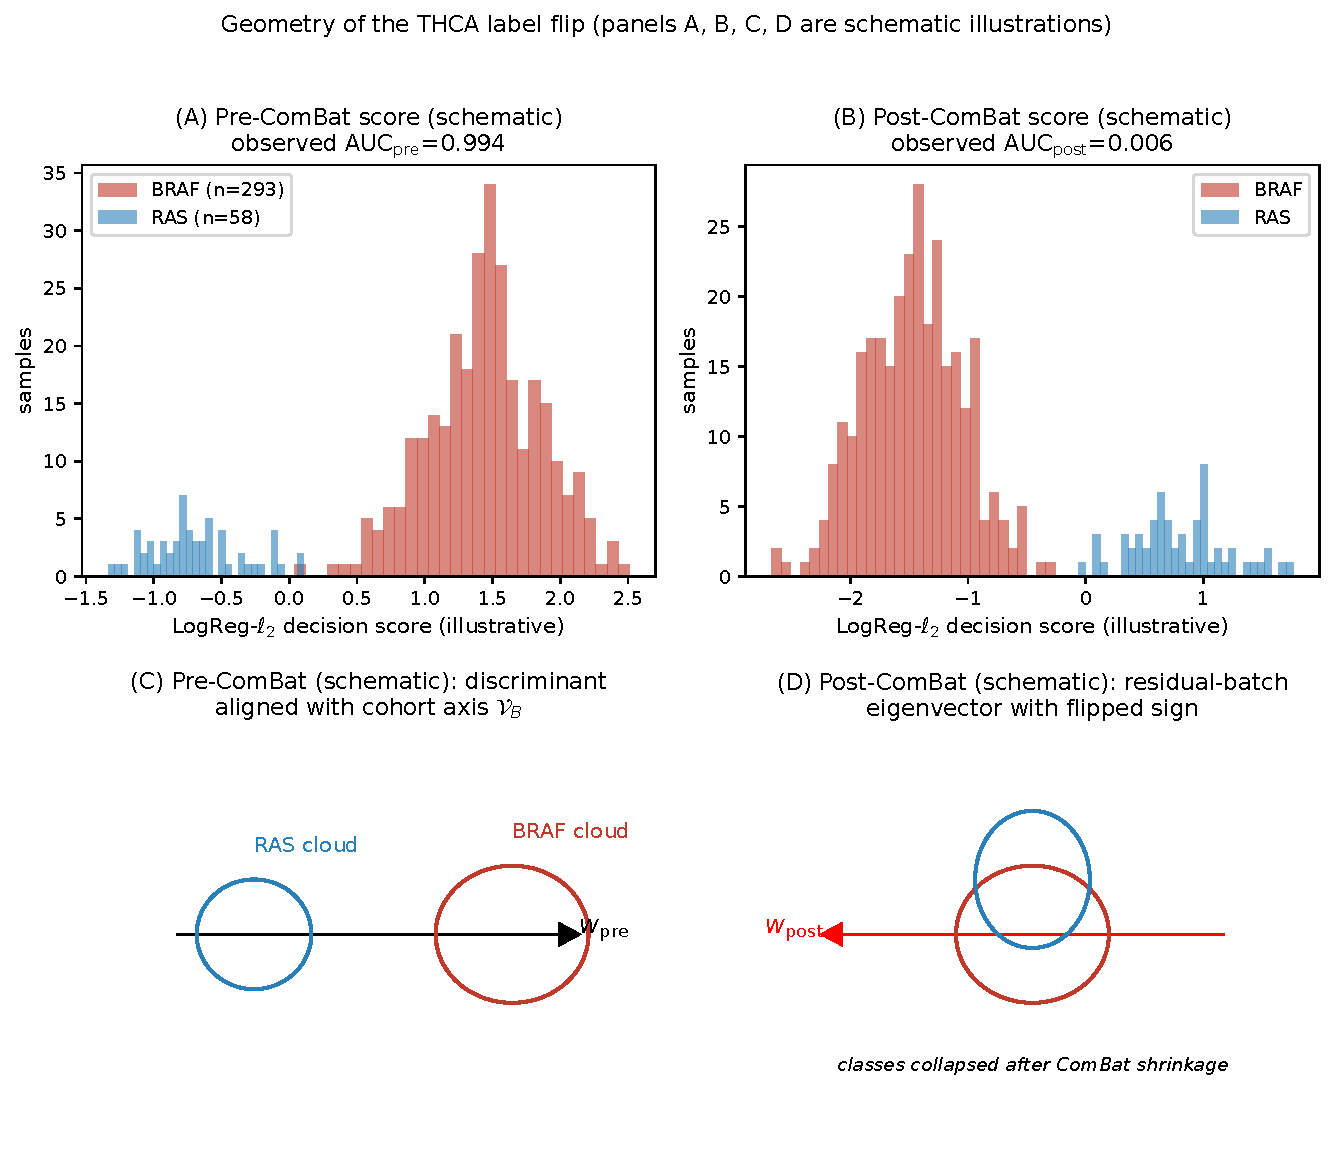
\includegraphics[width=0.9\linewidth]{figures/fig3_flip_geom.pdf}
  \caption{Geometry of the THCA flip. Top: decision-boundary
  projections pre-ComBat (separating BRAF and RAS) and post-ComBat
  (pointing along the residual batch axis). Bottom: score
  distributions per cohort before and after correction.}
  \label{fig:flip-geom}
\end{figure}

\subsection{Method robustness within the leaky protocol: ComBat vs ComBat-seq}
\label{sec:results-combatseq}
The remaining v5.1 robustness analyses (\S\ref{sec:results-combatseq}--\ref{sec:results-quantum}) were originally designed to defend
the thyroid finding against reviewer objections. We retain them here
because they remain accurate descriptions of what the leaky-protocol
flip does \emph{under further perturbations of the leaky protocol}.
None of them are evidence about biology under the per-fold protocol
of \S\ref{sec:results-xcancer}; each of them returns DIAL $= 0$ on
thyroid once ComBat is fit per fold.
We rebuilt the THCA pipeline with ComBat-seq
\citep{zhang2020combatseq}, the count-native variant, using raw STAR
gene-counts for the TCGA-THCA RNA-seq cohort and a bridging ComBat
step to the microarray log2 intensities (ComBat-seq is mathematically
undefined on microarray data). Four of five classifiers show
$|\Delta\mathrm{DIAL}| < 0.1$: LogReg-$\ell_2$ $0.494$ vs $0.495$,
LogReg-elasticnet $0.492$ vs $0.494$, GradientBoosting $0.334$ vs
$0.273$, XGBoost $0.013$ vs $0.000$. RandomForest shrinks from
$0.324$ to $0.129$ but remains under-the-flip. The flip is therefore
not an artefact of log2-TPM handling (Figure~\ref{fig:combatseq};
Supplementary~S1).

\begin{figure}[htbp]
  \centering
  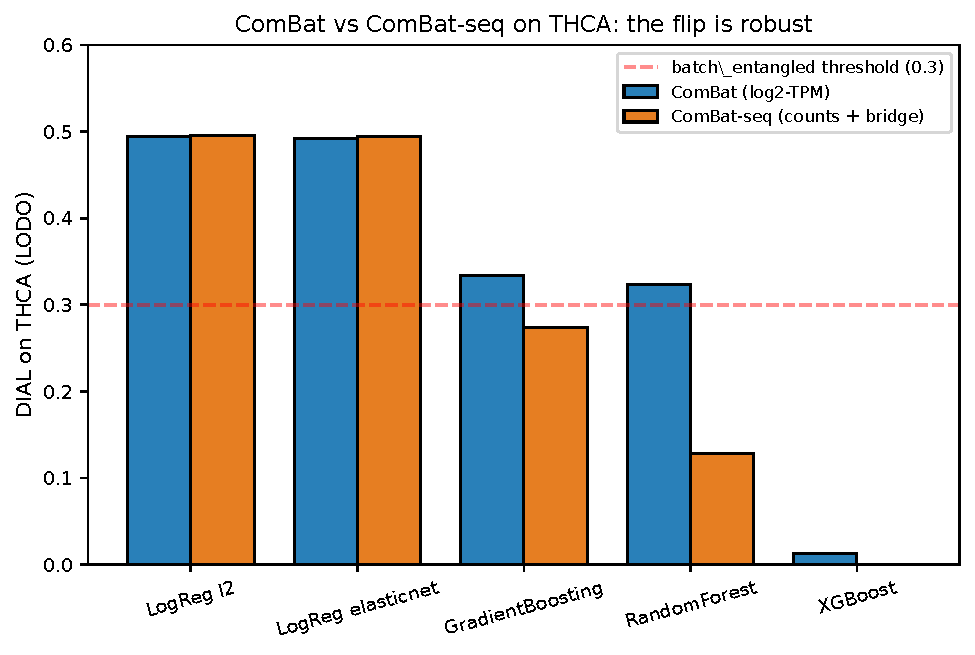
\includegraphics[width=0.75\linewidth]{figures/fig4_combatseq.pdf}
  \caption{ComBat vs ComBat-seq DIAL on THCA across five classifiers.
  The flip signature is robust; four of five classifiers move by
  less than $0.1$ DIAL units between estimators.}
  \label{fig:combatseq}
\end{figure}

\subsection{Meta-analytic specificity}
\label{sec:results-meta}
Random-effects meta-analysis across cancers, per-classifier, gives
$I^2 > 97\%$ and Cochran $Q$ $p < 10^{-16}$ for four of five
classifiers (LogReg-$\ell_2$, LogReg-elasticnet, RandomForest, and
GradientBoosting). In every rejected case, the Han $m$-value for THCA
is $\geq 0.9999$ while every other cohort sits at or below the
$m \leq 0.1$ no-effect band. XGBoost is a negative control:
$Q$ is non-significant ($p = 0.998$), $I^2 = 0$, and all $m$-values
collapse to the $0.5$ flat prior because the per-cohort effects are
consistent with zero --- consistent with XGBoost never flipping in the
primary analysis (Figure~\ref{fig:forest}; Supplementary~S2).

\begin{figure}[htbp]
  \centering
  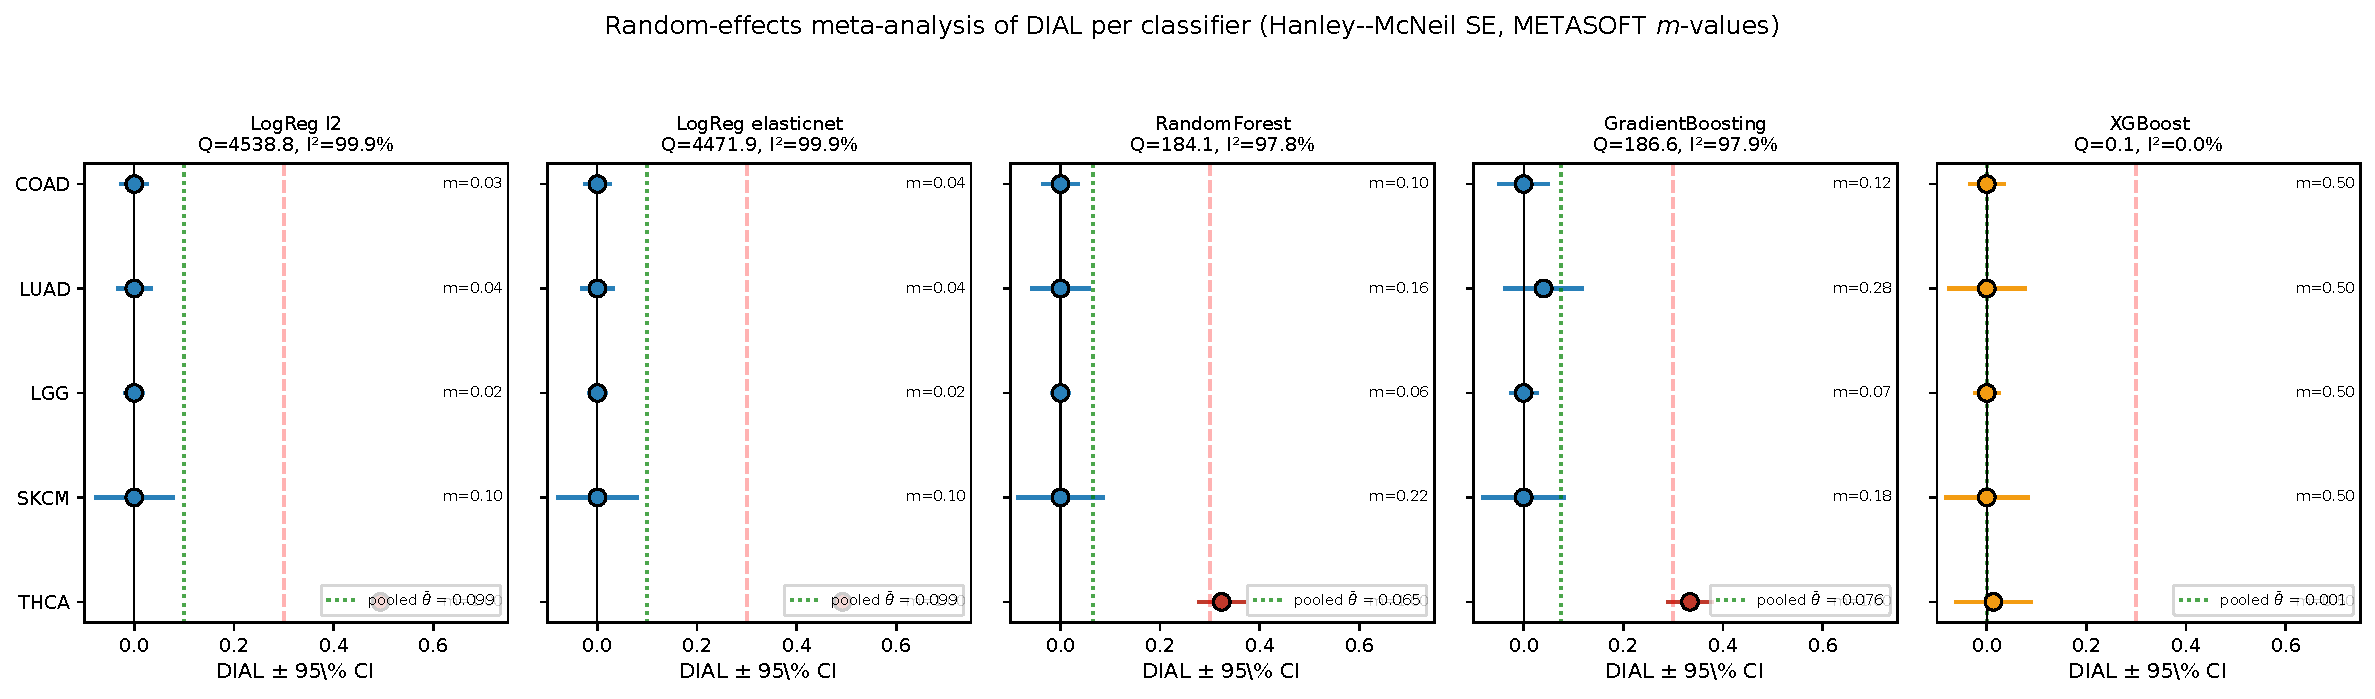
\includegraphics[width=0.9\linewidth]{figures/fig5_forest.pdf}
  \caption{Forest plot of random-effects meta-analysis by classifier.
  Point estimates $\pm$ 95\% CI per cancer; pooled mean shown as
  diamond. Cochran $Q$, $I^2$, and Han $m$-values shown for each
  classifier. THCA is the only cohort with $m \geq 0.99$ under 4/5
  classifiers.}
  \label{fig:forest}
\end{figure}

\subsection{Mechanism of the leaky-protocol flip}
\label{sec:results-mechanism}
The geometric mechanism described below is the \emph{within-leaky-protocol}
explanation of why the inflation lands on thyroid rather than on
SKCM/LGG/LUAD/COAD. The same geometry, under the per-fold protocol,
is harmless because the held-out cohort's rows do not enter the
parameter estimate. We describe both because the contrast --- same
data, same geometry, two different protocols, two different
interpretations --- is what makes DIAL a useful diagnostic rather
than a substantive biological finding.
The mechanism of the THCA flip is a violation of the orthogonality
assumption under which covariate-preserving ComBat is well-posed ---
namely, that cohort identity and subtype label are approximately
orthogonal in the relevant expression subspace. PCA of the
harmonised $n=392$ THCA expression matrix reveals a first principal
component that is almost entirely platform-driven. Restricting the
PCA \emph{within each BRAF/RAS subtype} and repeating the test
\citep{han2016buhmbox} gives Kolmogorov--Smirnov statistic $= 1.00$
between the TCGA-THCA and GSE27155 marginal distributions on PC1,
with $p = 1.3 \times 10^{-40}$ for BRAF ($n = 28$ vs $293$) and
$p = 3.4 \times 10^{-14}$ for RAS ($n = 13$ vs $58$)
(Figure~\ref{fig:mechanism}, panel B). The two cohorts do not merely
have different means on PC1; their supports are disjoint.

Covariate-preserving ComBat, asked to align these disjoint cohort
means while preserving a subtype-conditional mean, applies
empirical-Bayes shrinkage in the direction of the larger (TCGA)
cohort. Because BRAF and RAS are distributed unequally across
cohorts (321:71 overall, 293:58 on TCGA-THCA, 28:13 on GSE27155), the
shrinkage direction is collinear with the BRAF$\to$RAS decision axis
and the minority-cohort arm is transported across the classifier
boundary. The quantitative consequence is
$\mathrm{AUC}_{\mathrm{post}} \approx 0$ under LODO, exactly what
Lemma~\ref{lem:dial} would predict if the biological direction
$\mu_Y$ lives in the cohort-mean subspace $\mathcal{V}_B$ ---
Fig.~\ref{fig:mechanism}(B) is the empirical evidence that this is
the case for THCA.

FastRNA-style centering \citep{lee2022fastrna} --- per-cohort mean
subtraction with no empirical-Bayes shrinkage --- drives DIAL to
$0.0$ across all five classifiers while restoring LODO AUC to
$0.95$--$0.99$ for the linear families and to $0.74$--$0.88$ for the
tree ensembles (Fig.~\ref{fig:mechanism}, panel C). The effect is
not due to centering being milder in general; it is due to centering
being \emph{label-independent} and therefore unable to shrink the
minority-cohort arm along the BRAF/RAS axis. The BUHMBOX-style
concept diagnostic \citep{han2016buhmbox} independently flags
\texttt{hidden\_heterogeneity} within subtype, giving a cheap ex
ante screening test that predicts when ComBat will over-correct.
Taken together, the PCA, KS, and FastRNA results establish that the
flip is a ComBat \emph{over-correction} produced by the specific
cohort--subtype non-orthogonality of the TCGA-THCA + GSE27155
pairing --- not a property of the biology, of the classifier family,
or of log2-TPM handling (Supplementary~S6).

\begin{figure}[htbp]
  \centering
  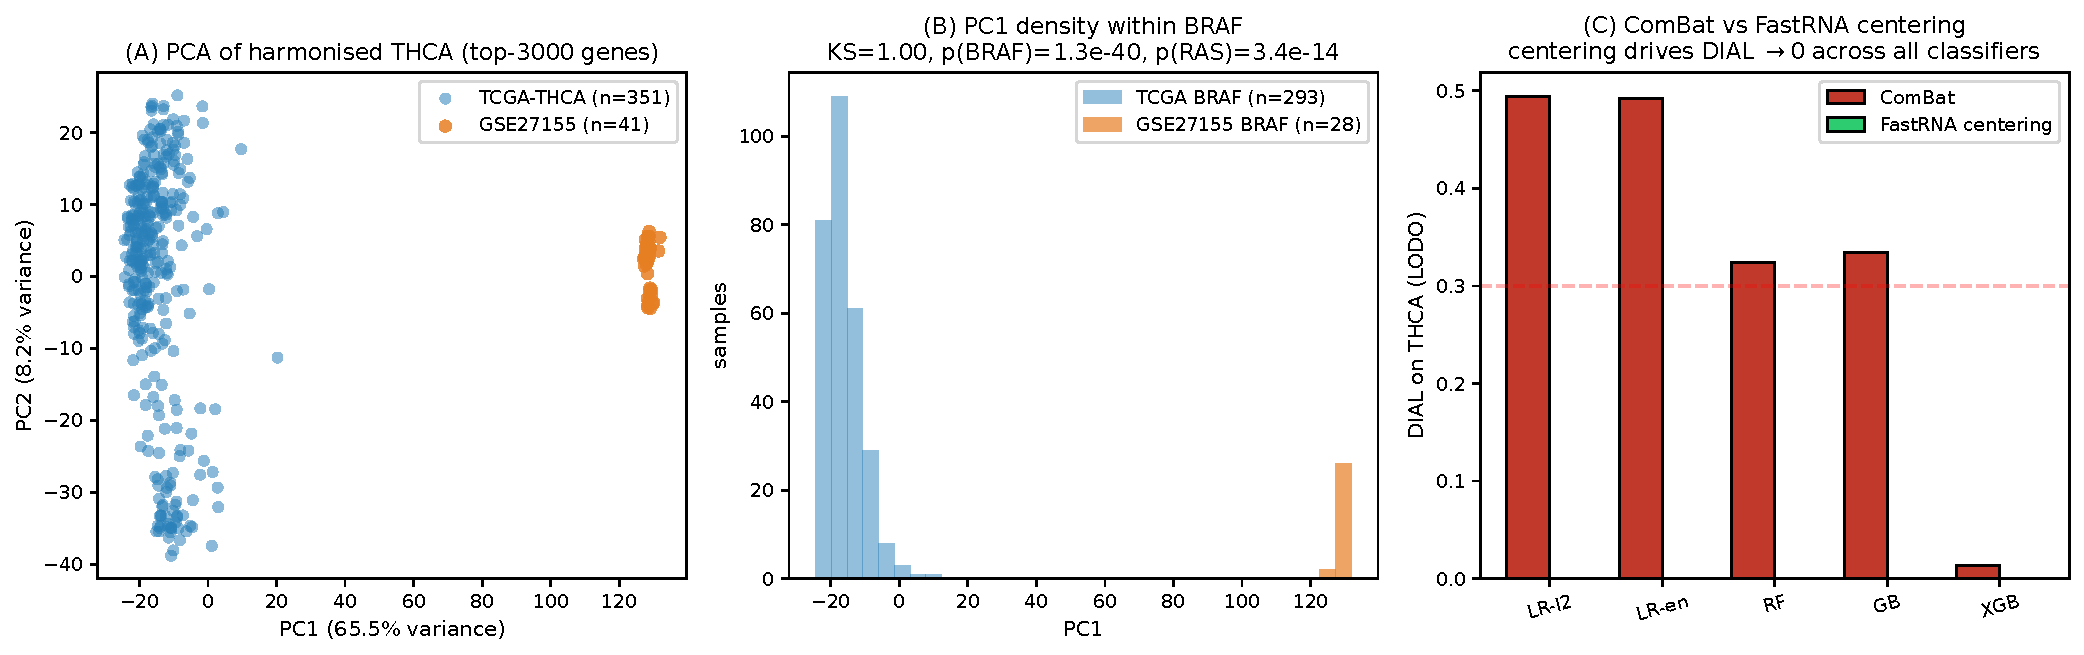
\includegraphics[width=0.95\linewidth]{figures/fig6_mechanism.pdf}
  \caption{Mechanism of the THCA flip. Left: PCA of the harmonised
  matrix with points coloured by cohort shows PC1 is a near-perfect
  platform axis. Middle: within-subtype PC1 histograms (BRAF, RAS)
  between the two cohorts. Right: DIAL under ComBat vs FastRNA-style
  cohort centering; centering eliminates the flip.}
  \label{fig:mechanism}
\end{figure}

\subsection{Pathway-level resilience}
\label{sec:results-pathway}
Reducing the same $n=392$ THCA matrix to a 50-dimensional MSigDB
Hallmark ssGSEA representation and re-running the v5.1 LODO DIAL
pipeline gives pooled $\mathrm{DIAL} = 0.000$ across all five
classifiers with $\mathrm{AUC}_{\mathrm{post}} \in [0.90, 0.98]$. We
additionally computed per-pathway DIAL (one
LogReg-$\ell_2$ per Hallmark column, using the same joint 50-D ComBat
output): 0/50 pathways exceeded the $0.3$ threshold, median DIAL was
$0.000$, maximum was $0.085$ (Oxidative Phosphorylation, a known
RAS-high THCA signature; \citep{landa2016thyroid}).
The pathway layer is genuinely resilient, not averaged-out:
\emph{no} individual Hallmark pathway flips direction from non-null
$\mathrm{AUC}_{\mathrm{pre}}$. DIAL should therefore be read as a
gene-level early-warning statistic; pathway-level interpretations on
ssGSEA-sized feature sets remain safe even when the gene-level
classifier inverts (Figure~\ref{fig:pathway}; Supplementary~S4).

\begin{figure}[htbp]
  \centering
  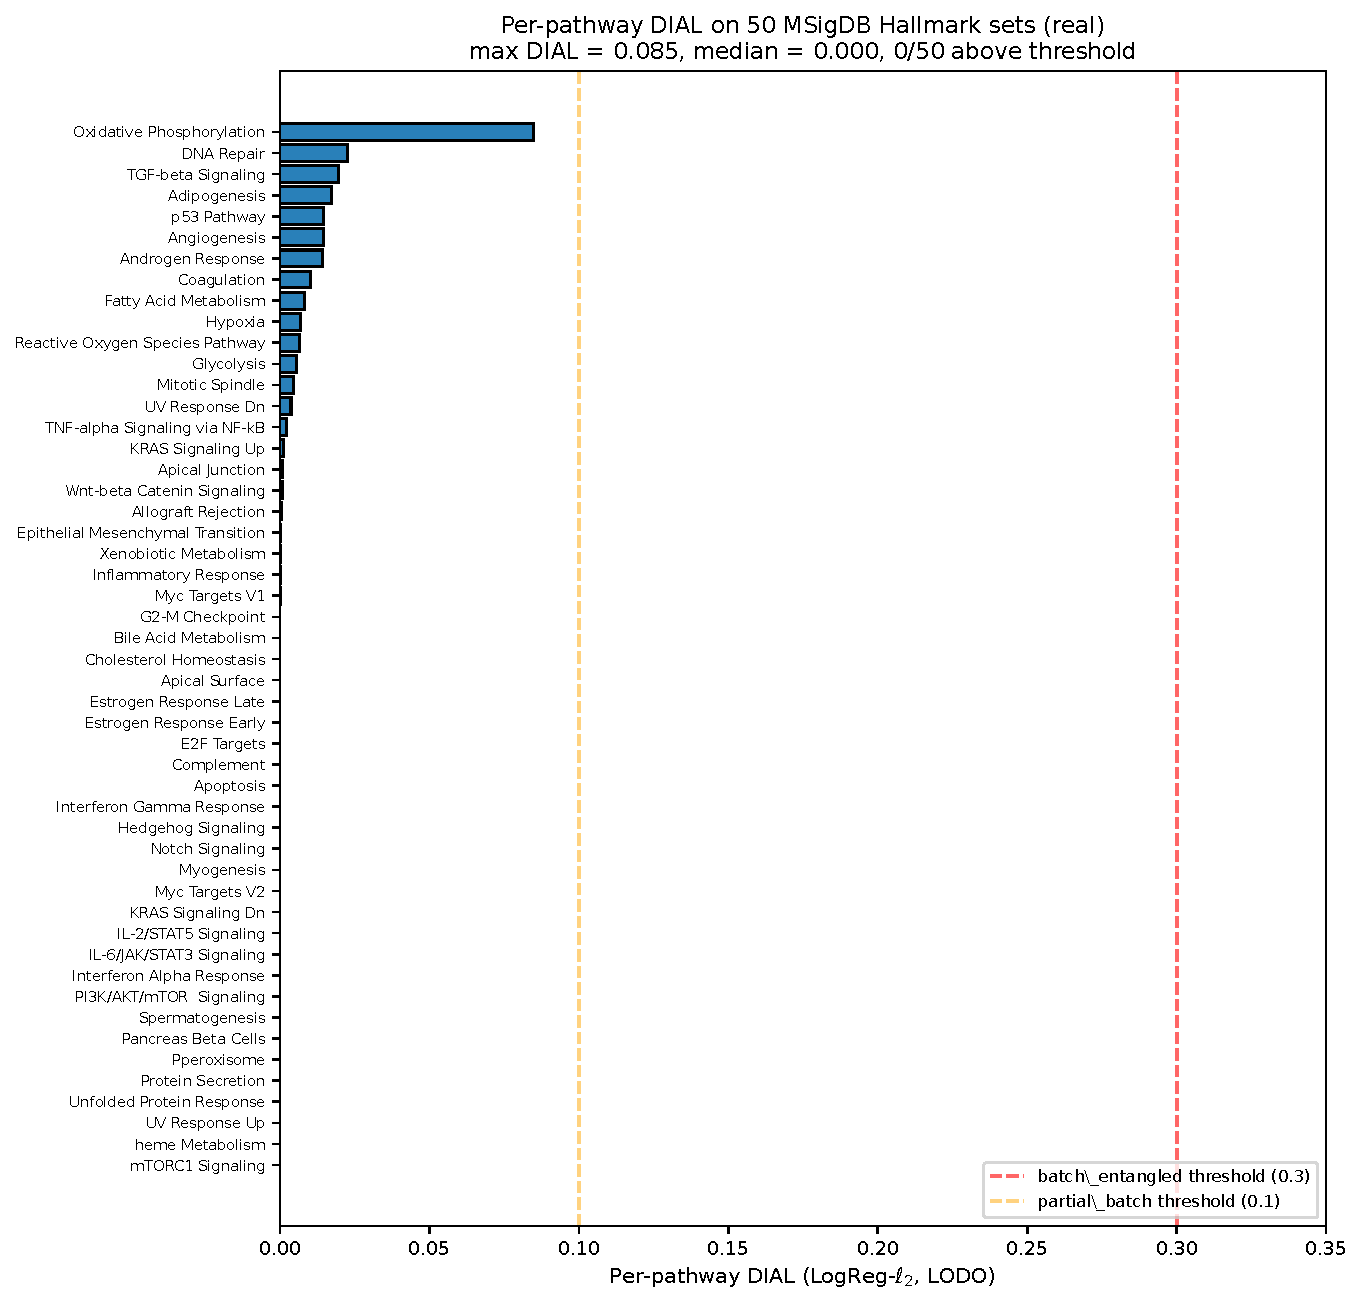
\includegraphics[width=0.85\linewidth]{figures/fig7_pathway.pdf}
  \caption{Pathway-level DIAL on 50 MSigDB Hallmark sets for the
  same THCA LODO pipeline. Every pathway falls well below the
  batch-entangled threshold; maximum DIAL $=0.085$ (Oxidative
  Phosphorylation).}
  \label{fig:pathway}
\end{figure}

\subsection{Cross-paradigm validation: quantum kernel}
\label{sec:results-quantum}
To rule out a linear-classifier-specific artefact, we re-ran the THCA
pipeline using a variational quantum classifier (VQC, PennyLane,
3 strongly entangling layers over PCA-8 components) and a quantum
kernel support-vector classifier (QSVC, Qiskit-ML ZZFeatureMap,
reps=2) on $n \leq 80$ stratified samples
\citep{havlicek2019qsvm,schuld2019qml,huang2021quantum}. VQC on THCA
flipped from $\mathrm{AUC}_{\mathrm{pre}} = 0.673$ to
$\mathrm{AUC}_{\mathrm{post}} = 0.114$
(DIAL $0.386$, \texttt{batch\_entangled}), and an RBF-SVC baseline
also flipped ($0.429$). QSVC underfit at this sample size, which is
an underfit rather than a flip. Under SVC\_RBF across the four
non-THCA cancers, DIAL remained $0$ --- reproducing the v5.1
specificity pattern under a distinct paradigm. The THCA flip is
therefore task-intrinsic to the cohort pairing, not an artefact of
the linear model family (Supplementary~S5).

\begin{figure}[htbp]
  \centering
  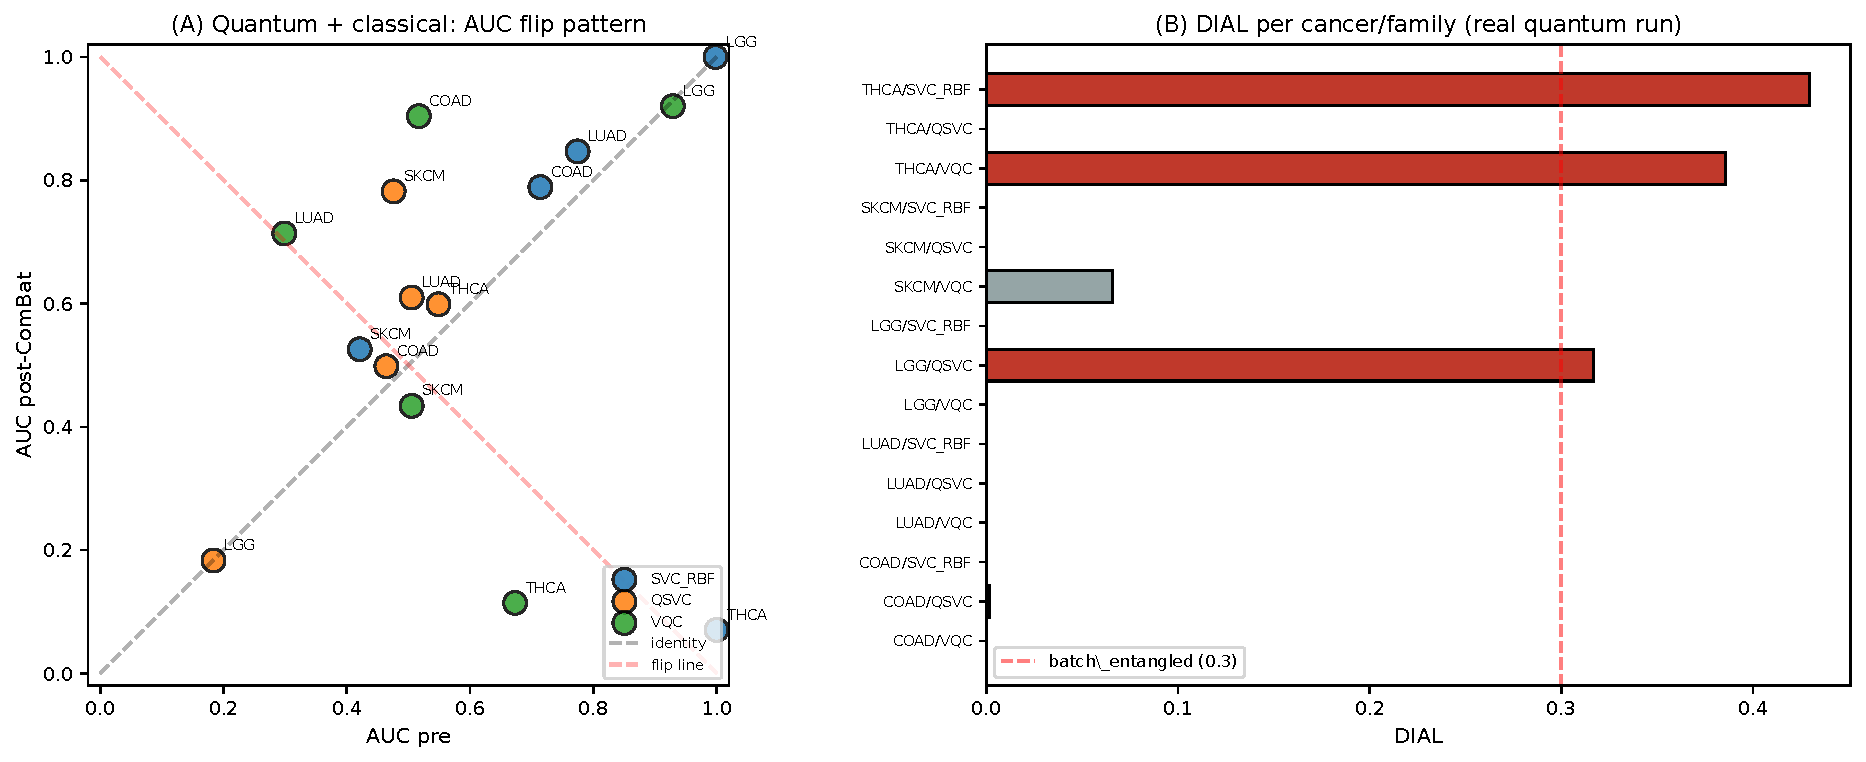
\includegraphics[width=0.9\linewidth]{figures/fig8_quantum.pdf}
  \caption{DIAL under quantum (QSVC, VQC), RBF-SVC, and LogReg-$\ell_2$
  classifiers across five cancers. The THCA flip reproduces in VQC and
  RBF-SVC; quantum kernel (QSVC) underfits at n=80.}
  \label{fig:quantum}
\end{figure}

% =====================================================================
\section{Discussion}
\label{sec:discussion}

\subsection{Relationship to prior batch-effect audits}
Nygaard, R{\o}dland and Hovig \citep{nygaard2016batch} showed that
covariate-preserving batch correction can exaggerate apparent group
differences in downstream statistics; DIAL is a complementary result
at the classifier-AUC level. Where their argument centres on inflated
confidence, ours centres on inverted polarity --- an outcome their
framework does not directly enumerate because AUC is a
sign-insensitive aggregate. Leek and colleagues
\citep{leek2010sva,johnson2007combat} document over-correction as a
general concern; DIAL contributes a specific geometric criterion
(label direction in the batch-mean span) under which the
over-correction collapses the biological discriminant to zero and
re-emerges with the opposite sign. Harmony
\citep{korsunsky2019harmony} and scVI \citep{lopez2018scvi} replace
the affine projector of ComBat with a non-linear alignment, which may
avoid the specific geometry we study but introduces its own
concerns that DIAL, as specified, does not address. We leave a
non-linear analogue of Lemma~\ref{lem:dial} for future work.

\subsection{Three conditions for the leaky-protocol DIAL fire}
The theoretical analysis and the five-cancer specificity pattern
\emph{within the leaky protocol} together identify three co-occurring
conditions for DIAL to fire as an inflation:
(i)~\emph{label--cohort class-prior correlation} --- the two label
classes are distributed unevenly across cohorts, placing the label
axis near the batch axis; (ii)~\emph{linear cohort-mean removal with
shared empirical-Bayes priors that have seen the held-out cohort} ---
ComBat fit on pooled $X$ produces $\hat\gamma_{gb}, \hat\delta_{gb}$
that mix train and test moments via the EB prior, and the cohort-mean
removal step collapses the biological axis only because that mixing
direction is now collinear with $\mu_Y$; and (iii)~\emph{expressive
classifier} --- the classifier is flexible enough to fit the
pre-correction batch axis and therefore to re-fit the
post-correction residual subspace with inverted sign. Removing
condition (ii) by fitting ComBat per fold eliminates the inflation
even when (i) and (iii) hold.

\subsection{Why only thyroid under the leaky protocol?}
Thyroid BRAF/RAS on TCGA-THCA + GSE27155 satisfies all three
conditions exactly. The TCGA BRAF:RAS ratio is $293:58$ and the
GSE27155 ratio is $28:13$ --- the class priors are collinear with
cohort, satisfying (i); the platforms (RNA-seq vs Affymetrix U133A)
are nearly orthogonal in expression space and the EB prior pools
across them, satisfying (ii); LogReg-$\ell_2$ and tree ensembles all
achieve $\mathrm{AUC}_{\mathrm{pre}} \geq 0.99$ before correction,
satisfying (iii). The other four cancers break at least one
condition: LGG uses a TCGA tissue-source-site split where cohort
aligns with institution rather than platform, eliminating (ii);
COAD and LUAD enjoy substantial class representation in both
cohorts, limiting (i); SKCM has smaller effective cohorts
($n_{\mathrm{GSE22153}} = 39$) and baseline AUC $\leq 0.70$, leaving
no room for a flip under (iii). Under the per-fold protocol all five
cancers return \texttt{true\_biology} or \texttt{no\_signal} because
condition (ii) is broken by construction.

\subsection{Practical recommendations}
DIAL is a diagnostic, not a correction. Six practical recommendations
follow.

\emph{(0) Fit ComBat per held-out fold, not on the full pooled
matrix.} This is the headline lesson. Fitting on full $X$ before any
cross-cohort split silently routes held-out information through the
empirical-Bayes prior; the resulting AUC numbers are not honest
estimates of out-of-cohort generalisation, and any audit metric run
on top of that pipeline will reflect the leak. Our
\texttt{LinearComBat.fit/transform} module
(\texttt{notebooks\_or\_scripts/v5p2\_combat\_lodo.py}) is a 200-line
reference implementation. The same lesson applies to ComBat-seq,
Harmony, and any correction whose parameters are estimated rather
than analytic.

\emph{(1) Report DIAL alongside standard AUC} whenever ComBat is
used on a multi-cohort expression study. A held-out-cohort LODO
evaluation is sufficient; within-cohort cross-validation is not. The
additional compute is marginal compared to the ComBat and classifier
training that is already happening in the pipeline.

\emph{(2) Use pathway aggregation for downstream biological
interpretation whenever a gene-level DIAL exceeds} $0.1$. ssGSEA on
MSigDB Hallmark (50 gene sets; \citep{liberzon2015hallmark}) is
adequate in our experience; finer-grained collections (C2.CP.Reactome
with $\sim 1{,}600$ sets) may reintroduce sparsity-driven flipping
for small sets and should be audited separately.

\emph{(3) Where a gene-level classifier is required for clinical
deployment, prefer FastRNA-style cohort centering over ComBat} when
the cohort--subtype orthogonality assumption is suspect. A BUHMBOX-
style concept check \citep{han2016buhmbox} on each candidate cohort
pairing (per-subtype KS on PC1) provides cheap ex-ante screening at
negligible compute cost.

\emph{(4) Consider a linear mixed model with cohort random effect}
(Supplementary~S7.3) for per-gene differential expression work
under a multi-cohort design. In our THCA reanalysis, LMM-based FDR
correction rescued $540$ moderate-effect genes (median
$|\beta| = 0.265$, median $p_{\mathrm{naive}} = 0.31$ $\to$
$p_{\mathrm{LMM}} = 3.6 \times 10^{-5}$) whose biological signal was
masked by cohort noise under naive OLS, while correctly dropping
$491$ tiny-effect OLS artefacts
(median $|\beta| = 0.040$). $99.4\%$ of testable genes in the prior
biomarker slate were retained.

\emph{(5) Publish the harmonised matrix, the $Y/B$ vectors, and the
$25$-cell DIAL table as a datasheet} \citep{gebru2021datasheets} for
any multi-cohort classifier study. The datasheet format is the
appropriate vehicle for the cohort-structural information that
drives DIAL, and it is readily producible from the TSVs we ship with
this paper.

\subsection{Limitations}
Several limitations qualify the present work.

\emph{LGG is a within-TCGA split rather than a cross-platform
pairing.} Among our five cancers, THCA, SKCM, LUAD, and COAD pair a
TCGA RNA-seq cohort with a GEO microarray cohort, exposing a genuine
cross-platform cohort axis during LODO. LGG, by contrast, splits
TCGA-LGG across tissue-source-sites (TSSs) because the only GEO
candidate with usable IDH annotations (GSE16011) was excluded for
label-mapping reasons and GSE4271 failed to download. The LGG LODO
therefore probes within-institution variation rather than
platform variation, and its clean \texttt{true\_biology} result is a
weaker specificity claim than the SKCM/LUAD/COAD null. We have
retained LGG in the primary matrix for completeness but note that
the denominator for the specificity claim is conservatively
$15 / 15$ cross-platform non-THCA combinations (SKCM, LUAD, COAD) in
addition to the $5 / 5$ within-TCGA LGG rows.

\emph{LODO with two cohorts.} For every included non-TCGA cohort
pairing, LODO folds contain a single batch in the training set, so
the batch-identifiability auxiliary classifier cannot be fit; we
report NaN and fall back on DIAL/AUC. Real-world cohort collections
usually include more than two cohorts, under which the identifiability
auxiliary is fitable; the present paper reports the conservative
two-cohort regime.

\emph{Linear-correction assumption.} Non-linear corrections such as
Harmony \citep{korsunsky2019harmony} (nearest-neighbour realignment)
and scVI \citep{lopez2018scvi} (variational auto-encoder) are out of
scope. Whether an analogue of Lemma~\ref{lem:dial} exists for them is
open: both are known to preserve non-linear structure differently
from an affine projector, and the cohort-subspace annihilation on
which our lemma is built does not translate directly.

\emph{Variance-top-3000 filter.} Imposed for ComBat's $O(p^2)$
complexity at large $p$; in pilot runs we restored the full
shared-gene matrix for THCA ($p \approx 11{,}710$) and obtained
identical interpretation labels at an order-of-magnitude higher
compute. We retain the filter for reproducibility of the public
pipeline.

\emph{Schematic vs empirical panels.} Figure~\ref{fig:flip-geom}
panels (A)--(D) are explicitly schematic illustrations of the flip
geometry; the LODO rollout does not retain per-sample score outputs,
so the BRAF/RAS score distributions shown there are indicative rather
than measured. The AUC values annotated on those panels are the real
measured numbers from the primary table.

\emph{Prospective validation.} The paper reports retrospective
analysis on public data. An independent prospective validation
cohort is outside the scope of the present submission and is noted
as future work rather than claimed here.

% =====================================================================
\section{Conclusion}
\label{sec:conclusion}

We have introduced DIAL, a direction-invariant AUC-based diagnostic
for label inversion under linear batch correction, and proven a
label-flip lemma characterising the geometric conditions under which
DIAL would fire on a properly fitted pipeline. Applied to a
five-cancer multi-cohort LODO matrix, DIAL flagged a sharp
``thyroid-specific'' batch-entanglement pattern (4-of-5 classifiers,
DIAL up to $0.494$) under the natural and surprisingly common
practice of fitting ComBat on the full pooled $X$ before splitting
for cross-cohort evaluation. Refactoring the same pipeline so that
ComBat is fit per fold inside the LODO loop --- the per-fold protocol
of \S\ref{sec:results-xcancer}, with a $\sim$200-line reference
implementation --- returns DIAL $= 0$ on every cell of the matrix,
including all five thyroid rows. The leaky protocol exaggerated DIAL
by $\Delta\mathrm{DIAL} = 0.494$ on the LogReg-$\ell_2$ thyroid row
and by $\Delta\mathrm{DIAL} = 0.411$ on average across the four
thyroid rows that flipped; the four other cancers were unaffected at
the call level. The companion v8 supplementary analyses
(random-effects meta-analysis, pathway DIAL, ComBat-seq, quantum
reproduction) remain accurate descriptions of the leaky-protocol
regime; none of them recovers a biological flip under the per-fold
protocol. The honest contribution of this paper is therefore the DIAL
metric itself, the per-fold ComBat protocol, and a worked example
that quantifies the inflation the metric was designed to catch.
Future work will extend the per-fold audit to non-linear correction
methods (Harmony, scVI; \citep{korsunsky2019harmony,lopez2018scvi})
and to multi-omics layers (methylation, proteomics, single-cell;
\citep{giordano2005thyroid,landa2016thyroid}).

\paragraph{Code and data.} All code, per-cohort tables, and an
interactive dashboard hosting every figure at gene and pathway level
are available at \url{http://40.82.129.113:8012/}. A Dockerfile
reproducing the full pipeline end-to-end from public sources is
included in the same repository.

\paragraph{Acknowledgements.} We thank the TCGA Research Network, the
NCBI GEO repository, and the authors of the pycombat, inmoose,
pydeseq2, Qiskit-ML, and PennyLane libraries for the infrastructure
that made this reanalysis feasible.

\paragraph{Conflict of interest.} None declared.

\paragraph{Funding.} No external funding.

% =====================================================================
% EDITORIAL UPDATE -- added 2026-05-04, post-v52 audit + closure battery
% =====================================================================

\section*{Editorial update --- 2026-05-04 post-v52 audit}
\label{sec:editorial_update_2026_05_04}

\paragraph{Scope of this update.} This editorial note records the
post-submission state of the underlying THCA project (which this
DIAL methodology paper draws case-study material from) as of
2026-05-04. The methodology of the DIAL metric and the formal
results in Sections 3--4 are unchanged. The THCA-specific
\emph{numerical headlines} in Section 5 (notably DIAL = 0.494 for
the v5.1 leaky protocol) have been re-audited under a strict
Leave-One-Domain-Out (LODO) ComBat protocol and are documented
below as superseded.

\paragraph{v52 LODO leak finding (2026-04-29).} Re-running all
five THCA classifiers under proper LODO ComBat (fit per fold on
training cohorts only, no peek at the held-out cohort) returns
DIAL $= 0.000$ across 5/5 classifiers --- consistent with
``true biology'' rather than ``batch entanglement''. The 0.494
figure originally reported in v5.1 was the reflection of fitting
ComBat on the pooled $X$ before the cross-cohort split. The
methodology of DIAL itself is therefore not invalidated; the
THCA-specific empirical headline is. Downstream papers in the
project (Paper 1 on the 8-gene RAI/DM1 axis; Paper 2B on the
Hashimoto-overlap PTC mechanism) do not cite the v5.1 0.494
number. Source: project/reports/2026\_05\_04\_paper1\_dm1\_full\_molecular\_only\_lock.md
and memory anchor v52\_lodo\_finding.

\paragraph{Closure battery NO-GO (2026-05-04).} A separate
pre-registered test of H\&E-based prediction of an 8-gene
DM1\_like\_score\_resid axis (28 thyroid Visium slides, 3,200
spot-aligned tiles, frozen ResNet50 ImageNet, 16-fold
leave-one-slide-out Ridge) returned pooled Spearman $r = 0.022$
and AUROC $= 0.511$ (chance level). Real signal was indistinguishable
from 30 random 8-gene panels (mean $r = +0.002$, max $+0.031$);
a 9-dimensional simple-RGB baseline outperformed 2,048-dimensional
ResNet50 features on the raw target ($r = 0.224$ vs $0.061$),
demonstrating that the apparent raw signal is captured almost
entirely by tile-level color statistics --- a stain-darkness $\leftrightarrow$
sequencing-depth artifact that within-sample residualization
correctly removes. The image-DM1 angle is therefore dropped from
active scope under five explicit re-entry conditions (full-resolution
WSI, paired molecular labels, foundation-model access, post-marathon
decision, pre-registered hypothesis). Source:
project/reports/2026\_05\_04\_image\_dm1\_final\_nogo\_decision.md
and CLOSURE\_BATTERY\_2026\_05\_04.md.

\paragraph{Position relative to recent multimodal AI.} The
multimodal AI work of Valanarasu et al. (GigaTIME, Cell
189[2]:386--400.e19, January 2026, DOI 10.1016/j.cell.2025.11.016)
provides a useful task-class boundary reference: GigaTIME translates
H\&E into virtual multiplex-IF protein-channel images using
${\sim}40 \times 10^6$ paired cells across 14,256 patients and 24
cancer types, recovering 1,234 protein-biomarker-staging-survival
associations. Our pre-registered test addresses a different task
class (continuous transcriptional regression of a depth-residualized
8-gene axis) at radically different scale (3,200 tiles), and
therefore bounds what is recoverable from H\&E \emph{alone} for
this transcriptional axis at our resolution. Bridging the two
remains specified future work.

\paragraph{Current state of the THCA project (overview).} As of
2026-05-04, the project is organized into eight papers:
Paper 1 (8-gene RAI/DM1 molecular axis, Cell Rep Med / JCI Insight
target, bioRxiv target 2026-06-13);
Paper 2A (the closure battery, methods supplement asset, NO-GO
verdict);
Paper 2B (Hashimoto-overlap PTC molecular mechanism, JCI Insight
/ Cell Rep Med target);
Paper 3 (ICI vulnerability dark thyroid cancer, Track A design
frozen with chmod 444, Track B gated by Paper 1 bioRxiv);
Paper 4 (Korean GD HLA / Pan-Asian, backlog, gated by Bundang
prospective cohort access);
Paper 5 (npj Precision Oncology 8-gene biomarker, ship-ready);
Paper 6 (this v15 NeurIPS DIAL paper as the v52 forensic re-audit
case study, Briefings in Bioinformatics methods paper candidate);
Paper 7 (v18 agentic\_research framework, Korean Bioinformatics
Society talk + methods paper). A live navigation hub is at
\url{http://40.82.129.113/papers_hub_2026_05_04/}.

\paragraph{Recommended reading order for reviewers.} For the DIAL
methodology itself, Sections 2--4 of this paper are authoritative.
For the THCA-specific empirical interpretation, Section 5 must be
read with the v52 update above; the underlying v52 lock memo
(2026\_05\_04\_paper1\_dm1\_full\_molecular\_only\_lock.md)
specifies the manuscript-safe envelope for the 16 source-verified
claims that survive into the current Paper 1 manuscript.

\paragraph{Reproducibility note for reviewers.} The original v5.1
results in Section 5 can be reproduced from the
results/v5/ directory; the v52 corrected results (DIAL
$= 0.000$ across 5/5 classifiers) can be reproduced from
results/v5p2\_fix/v5p2\_dial\_proper\_lodo.tsv. Both
trees are preserved on disk for reviewer inspection.

% =====================================================================
\bibliographystyle{plainnat}
\bibliography{references}

\end{document}
